\chapter{Planning and Methodology}

In order to accomplish the Master's thesis during the established period of eight months, the following plan will be followed:
\begin{enumerate}[label=\textbf{\arabic*}.]
    \item \textbf{Exploratory phase:} this period of time will consist in searching and studying the literature related to the research field in order to build a solid theoretical framework on which support the rest of the investigation. Even though this process is presented as a isolated task, it is an fundamental activity that will be executed continuously throughout the whole project.
    \item \textbf{First contact with the technology:} after having reviewed the first phase of the state of art and checked the advantages or limitations of each architecture, the first empirical tests will be done. These experiments will serve to for a better understanding of the literature read in the exploratory phase and to observe how they behave with the gathered sample data.
    \item \textbf{Specification and design of the solution:} in this phase, based on the knowledge gathered from the empirical tests in the last point and the relevant literature that has been constantly read, the requirements of the solution that best results can achieve for this research topic will be specified.
    \item \textbf{Design of the functional prototype and evaluation:} after the requirements gathering, during this task, a prototype that justify all the steps followed this far will be developed, and evaluate its performance.
    \item \textbf{Thesis document writing:} Finally all the relevant knowledge that has been required to complete this research will be gathered, the procedure to develop the system will be described and the conclusion and future work on this topic will be written down altogether, resulting in this master's thesis document, that will be refined until its laster submission and defense.
\end{enumerate}

Previously defined tasks will be executed according to the next schedule diagram:

\begin{figure}[!htp]
  \center
  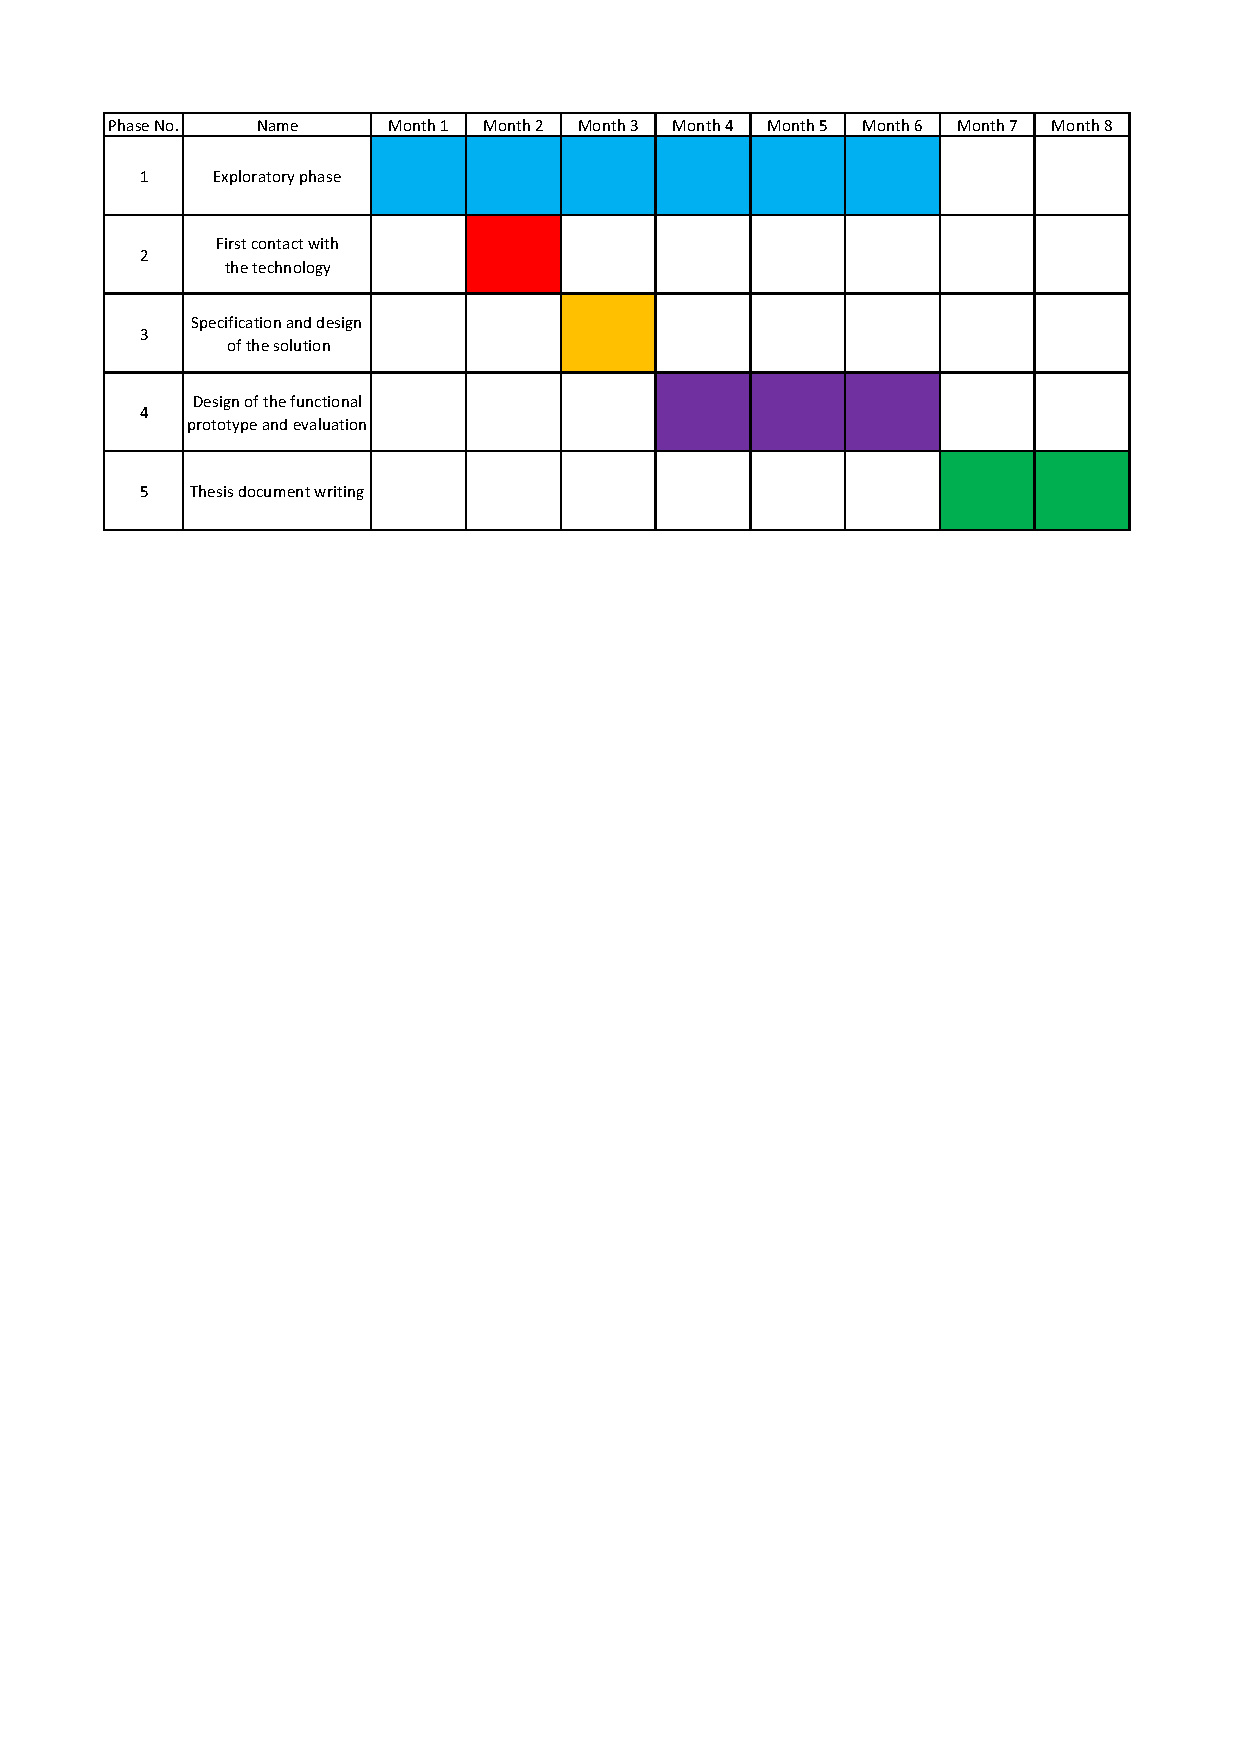
\includegraphics[width=1\textwidth]{figures/schedule}
  \caption{Schedule}
  \label{fig:schedule}
\end{figure}

\FloatBarrier

The figure \ref{fig:methodology} illustrates the methodology used during the investigation process, in which the results obtained from the prototypes might not be satisfactory or could lead to formulate new questions. To solve those doubts a redesign of the system may be needed. In addition, after reporting the results to project supervisor, new relevant information might be provided. This information has to be added to the knowledge obtained from previous state of the art review and reanalyze if the proposed solution requirements are still valid. 

\begin{figure}[!htp]
  \center
  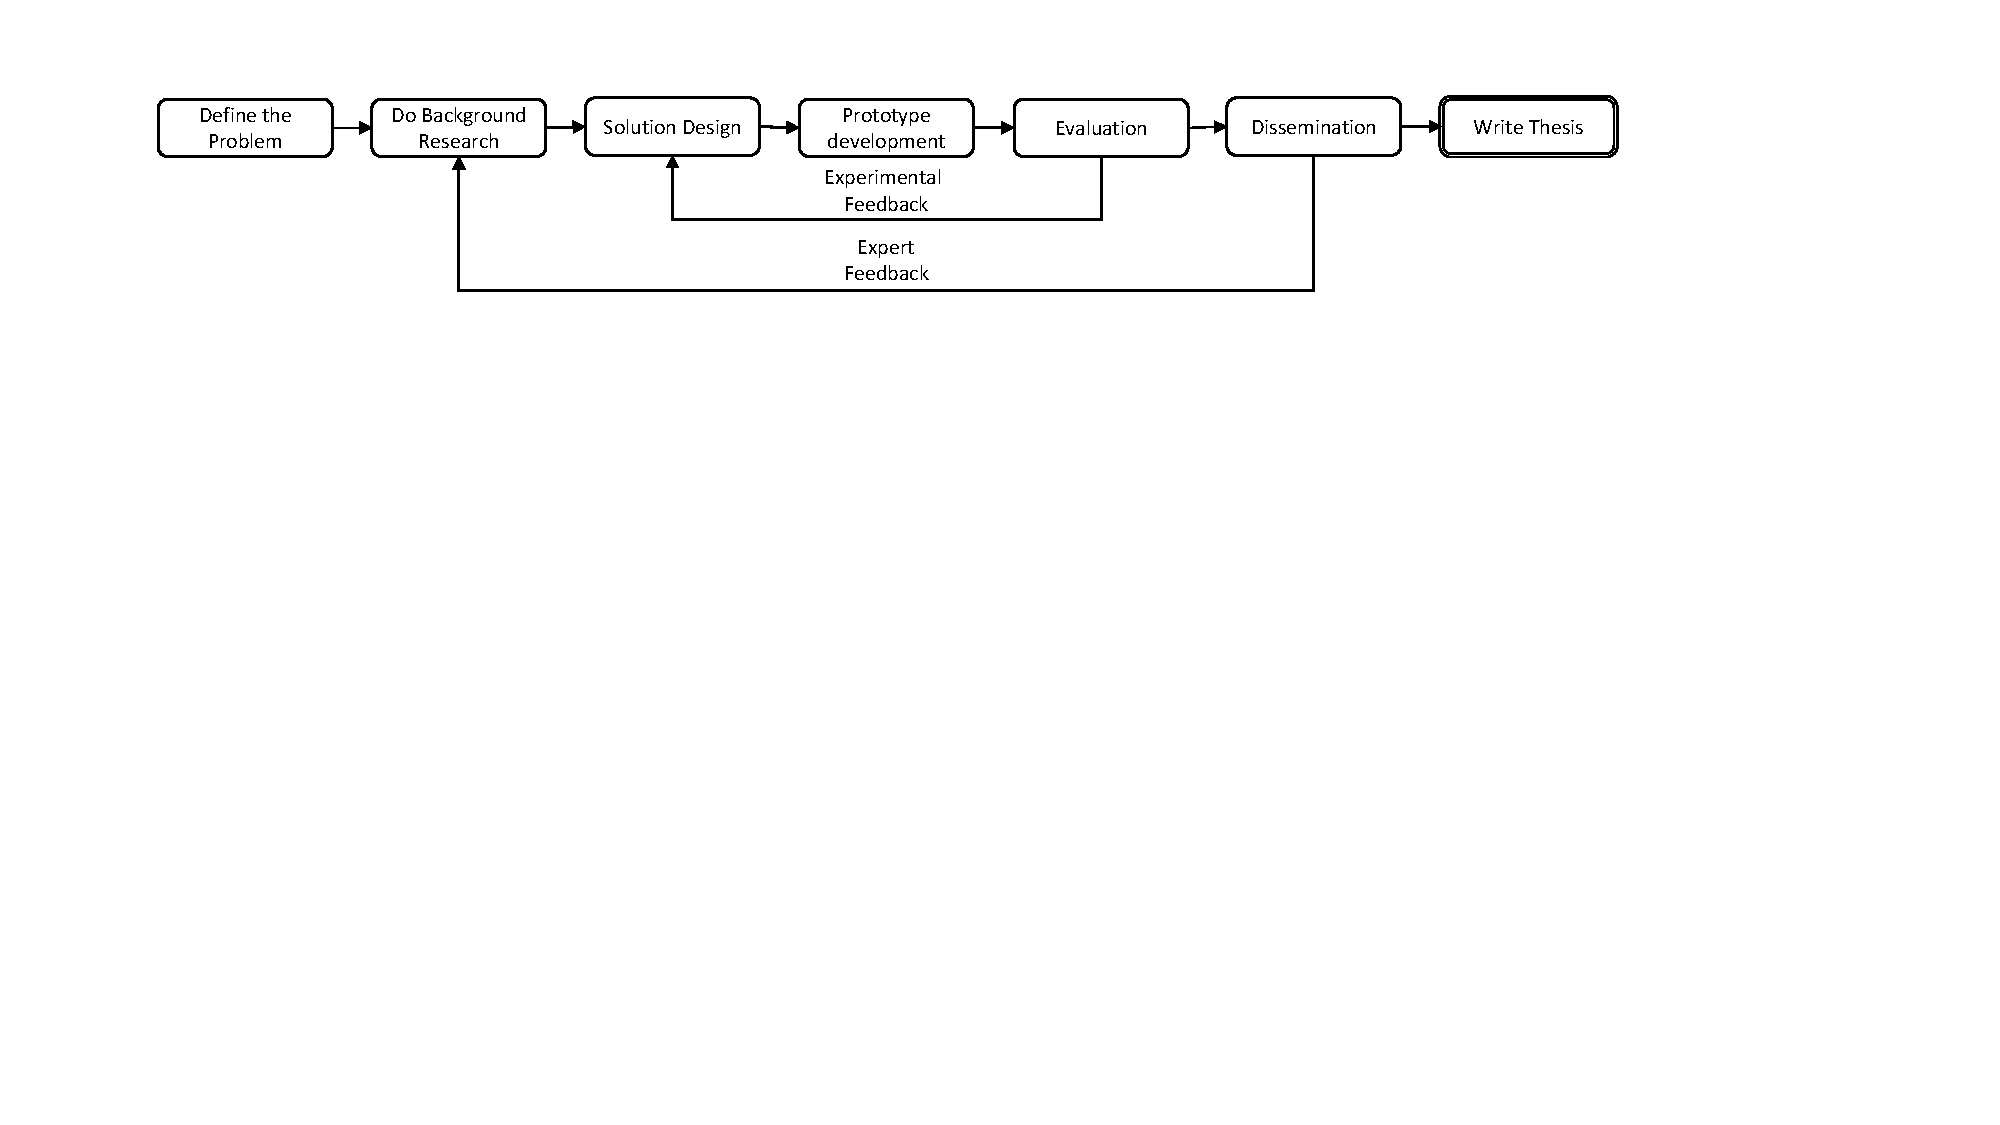
\includegraphics[width=1\textwidth]{figures/scientific_methodology}
  \caption{Methodology}
  \label{fig:methodology}
\end{figure}